\documentclass{tufte-handout}

\title{Notes on SwAV\thanks{Caron, Mathilde, et al. "Unsupervised learning of visual features by contrasting cluster assignments." arXiv preprint arXiv:2006.09882 (2020).}}

\author[The Tufte-LaTeX Developers]{Seri Lee}

%\date{28 March 2010} % without \date command, current date is supplied

%\geometry{showframe} % display margins for debugging page layout

\usepackage{graphicx} % allow embedded images
  \setkeys{Gin}{width=\linewidth,totalheight=\textheight,keepaspectratio}
  \graphicspath{{../images}} % set of paths to search for images
\usepackage{amsmath}  % extended mathematics
\usepackage{booktabs} % book-quality tables
\usepackage{units}    % non-stacked fractions and better unit spacing
\usepackage{multicol} % multiple column layout facilities
\usepackage{lipsum}   % filler text
\usepackage{fancyvrb} % extended verbatim environments
  \fvset{fontsize=\normalsize}% default font size for fancy-verbatim environments
% \usepackage{cite}
\usepackage{amsmath, amssymb, amsfonts}
\usepackage[ruled, vlined]{algorithm2e}
\usepackage{geometry}
\usepackage[utf8]{inputenc}
\usepackage{pgfplots}
\usepackage{textcomp}
\usepackage{xcolor}
\usepackage{verbatim}
\usepackage{tikz}

% \pgfplotsset{width=10cm, compat=1.9}
% Standardize command font styles and environments
\newcommand{\doccmd}[1]{\texttt{\textbackslash#1}}% command name -- adds backslash automatically
\newcommand{\docopt}[1]{\ensuremath{\langle}\textrm{\textit{#1}}\ensuremath{\rangle}}% optional command argument
\newcommand{\docarg}[1]{\textrm{\textit{#1}}}% (required) command argument
\newcommand{\docenv}[1]{\textsf{#1}}% environment name
\newcommand{\docpkg}[1]{\texttt{#1}}% package name
\newcommand{\doccls}[1]{\texttt{#1}}% document class name
\newcommand{\docclsopt}[1]{\texttt{#1}}% document class option name
\newenvironment{docspec}{\begin{quote}\noindent}{\end{quote}}% command specification environment

\begin{document}

\maketitle% this prints the handout title, author, and date

\begin{abstract}
Unsupervised image representations have significantly reduced the gap with supervised pretraining, notably with the recent achievements of contrastive learning methods.
These contrastive methods typically work online and rely on a large number of explicit pairwise feature comparisons, which is computationally challenging.
In the paper mentioned above, they propose an online algorithm, SwAV, that takes advantage of contrastive methods without requiring to compute pairwise comparisons.

Specifically, our method simultaneously clusters the data while enforcing consistency between cluster assignments produced for different augmentations (or ``views'') of the same image,
instead of computing features directly as in contrastive learning.

Simply out, we use a ``swapped'' prediction mechanism where we predict the code of a view from the representation of another view.

Our method can be trained with large and small batches and scale to unlimited amounts of data.
Compared to previous method, our method is more memory efficient since it does not require a large memory bank or a special momentum network.

In addition, we also propose a new data augmentation stratey, $multi-crop$, that uses a mix of views with different resolutions in place of two full-resolution views, without increasing the memory or compute requirements.

We validate our findings by achieving 75.3\% top-1 accuracy on ImageNet with ResNet-50, as well as surpassing supervised pretraining on all the considered transfer tasks.
\end{abstract}

  \begin{table}[ht]
    \centering
    \fontfamily{ppl}\selectfont
    \begin{tabular}{cccc}
      \toprule
      Method & Architecture & Parameter & top-1 accuracy \\
      \midrule
      MoCo & ResNet50 & 24 & 60.6 \\
      PIRL & ResNet50 & 24 & 63.6 \\
      SIMCLR & ResNet50 & 24 & 70.0 \\
      SwAV & ResNet50 & 24 & 75.3 \\
      \bottomrule
    \end{tabular}
    \caption{\textbf{Linear classification on ImageNet}. Top-1 accuracy for linear models trained on frozen features from different self-supervised methods.}
    \label{tab:normaltab}
    %\zsavepos{pos:normaltab}
  \end{table}
%\printclassoptions

\section{Introduction}\label{sec:introductions}
\newthought{Many recent state-of-the-art methods} build upon the instance discrimination task that considers each image of the dataset (``instance'')
and its transformations as a separate class.
This task yields representations that are able to discriminate between different images, while achieving some invariance to image transformations.
Recent self-supervised methods that use instance discrimination rely on a combination of two elements: (1) a contrastive loss and (2) a set of image transformations.

The contrastive loss removes the notion of instance classes by direcly mapping image features while the image transformations define the invariances encoded in the features.
Both elements are essential to the quality of the resulting network. 

\begin{marginfigure}
  \begin{center}
  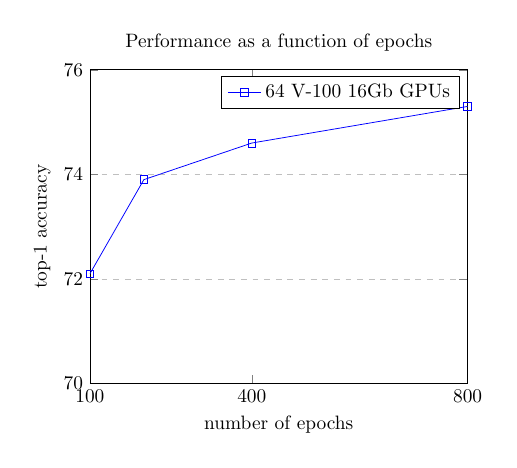
\begin{tikzpicture}[scale=0.7]
    \begin{axis}[
        title={Performance as a function of epochs},
        xlabel={number of epochs},
        ylabel={top-1 accuracy},
        xmin=100, xmax=800,
        ymin=70, ymax=76,
        xtick={100, 400, 800},
        ytick={70, 72, 74, 76},
        ymajorgrids=true,
        grid style=dashed,
    ]
    
    \addplot[
        color=blue,
        mark=square,
        ]
        coordinates {
        (100, 72.1)(200, 73.9)(400, 74.6)(800, 75.3)
        };
        \legend{64 V-100 16Gb GPUs}
        
    \end{axis}
    \end{tikzpicture}
  \end{center}
    \caption{\textbf{Performance as a function of epochs}.Comparing SwAV models trained with different number of epochs and reporting their running time.}
  \label{fig:marginfig}
  \end{marginfigure}

The contrastive loss explicitly compares pairs of image representations to push away representations from different images while pulling together those transformations, or views, of the same image.

Since computing all the pairwise comparisons on a large dataset is not practical, most implementations approximate the loss by reducing the number of comparisons to random subsets of images during training.
An alternative to approximate the loss is to approximate the task-that is to relax the instance discrimination problem.
For example, clustering-based methods discriminate between groups of images with similar features instead of individual images.

The objective in clustering is tractable, but it does not scale well with the dataset as it requires a pass over the entire dataset to form image ``codes'' (\textit{i.e.}, cluster assignments) that are used as targets during training.
In this work, we use a different paradigm and propose to compute the codes online while enforcing consistency between codes obtained from views of the same image.

Comparing cluster assignments allows to contrast different image views while not relying on explicit pairwise feature comparisons.
Specifically, we propose a simple ``swapped'' prediction problem where we predict the code of a view from the representation of another view.

We learn features by Swapping Assignments between multiples Views of the Same Image (SwAV). The features and codes are learned online, allowing our method to scale to potentially unlimited amounts of data.

\begin{figure}
  \includegraphics[scale=5]{instance}
%  \checkparity This is an \pageparity\ page.%
  \caption{Contrastive instance learning.
  \emph{the features from different transformations of the same images are compared directly to each other.}}
  \label{fig:textfig}
  %\zsavepos{pos:textfig}
  \setfloatalignment{b}
\end{figure}

\begin{figure}
  \includegraphics[scale=5]{swav}
%  \checkparity This is an \pageparity\ page.%
  \caption{SwAV.
  \emph{We first obtain ``codes'' by assigning features to prototype vectors. Then solve a ``swapped'' prediction problem wherein the codes obtained from one data augmented view are predicted using the other view.
  Prototype vectors are learned along with the ConvNet parameters by backpropagation.}}
  \label{fig:textfig}
  %\zsavepos{pos:textfig}
  \setfloatalignment{b}
\end{figure}

\section{Related Work}\label{sec:related-work}
\subsection{Instance and contrastive learning}\label{sec:instance-and-contrastive-learning}

Besides our online clustering-based method, we also propose an improvement to the image transformations.
Most contrastive methods compare one pair of transformations per image, even though there is evidence that comparing more views during training improves the resulting model.
In this work, we propose $multi-crop$ that uses smaller-sized images to increase the number of views while not increasing the memory or computational requirements during training.
We also observe that mapping small parts of a scene to more global views significantly boosts the performance.

Directly working with downsized images introduces a bias in the features, which can be avoided by using a mix of different sizes.
Our strategy is simple, yet effective, and can be applied to many self-supervised methods with consistent gain in performance.

They validate their contributions by evaluating their protocol on several standard self-supervised benchmarks.

%\begin{docspec}
%  \doccmd{newthought\{In his later books\}, Tufte starts\ldots}
%\end{docspec}

\subsection{Sidenotes}\label{sec:sidenotes}
One of the most prominent and distinctive features of this style is the
extensive use of sidenotes.  There is a wide margin to provide ample room
for sidenotes and small figures.  Any \Verb|\footnote|s will automatically
be converted to sidenotes.\footnote{This is a sidenote that was entered
using the \texttt{\textbackslash footnote} command.}  If you'd like to place ancillary
information in the margin without the sidenote mark (the superscript
number), you can use the \Verb|\marginnote| command.\marginnote{This is a
margin note.  Notice that there isn't a number preceding the note, and
there is no number in the main text where this note was written.}

The specification of the \Verb|\sidenote| command is:
\begin{docspec}
  \doccmd{sidenote[\docopt{number}][\docopt{offset}]\{\docarg{Sidenote text.}\}}
\end{docspec}

Both the \docopt{number} and \docopt{offset} arguments are optional.  If you
provide a \docopt{number} argument, then that number will be used as the
sidenote number.  It will change of the number of the current sidenote only and
will not affect the numbering sequence of subsequent sidenotes.

Sometimes a sidenote may run over the top of other text or graphics in the
margin space.  If this happens, you can adjust the vertical position of the
sidenote by providing a dimension in the \docopt{offset} argument.  Some
examples of valid dimensions are:
\begin{docspec}
  \ttfamily 1.0in \qquad 2.54cm \qquad 254mm \qquad 6\Verb|\baselineskip|
\end{docspec}
If the dimension is positive it will push the sidenote down the page; if the
dimension is negative, it will move the sidenote up the page.

While both the \docopt{number} and \docopt{offset} arguments are optional, they
must be provided in order.  To adjust the vertical position of the sidenote
while leaving the sidenote number alone, use the following syntax:
\begin{docspec}
  \doccmd{sidenote[][\docopt{offset}]\{\docarg{Sidenote text.}\}}
\end{docspec}
The empty brackets tell the \Verb|\sidenote| command to use the default
sidenote number.

If you \emph{only} want to change the sidenote number, however, you may
completely omit the \docopt{offset} argument:
\begin{docspec}
  \doccmd{sidenote[\docopt{number}]\{\docarg{Sidenote text.}\}}
\end{docspec}

The \Verb|\marginnote| command has a similar \docarg{offset} argument:
\begin{docspec}
  \doccmd{marginnote[\docopt{offset}]\{\docarg{Margin note text.}\}}
\end{docspec}

\subsection{References}
References are placed alongside their citations as sidenotes,
as well.  This can be accomplished using the normal \Verb|\cite|
command.\sidenote{The first paragraph of this document includes a citation.}

The complete list of references may also be printed automatically by using
the \Verb|\bibliography| command.  (See the end of this document for an
example.)  If you do not want to print a bibliography at the end of your
document, use the \Verb|\nobibliography| command in its place.  

To enter multiple citations at one location,\cite{Tufte2006,Tufte1990} you can
provide a list of keys separated by commas and the same optional vertical
offset argument: \Verb|\cite{Tufte2006,Tufte1990}|.  
\begin{docspec}
  \doccmd{cite[\docopt{offset}]\{\docarg{bibkey1,bibkey2,\ldots}\}}
\end{docspec}

\section{Figures and Tables}\label{sec:figures-and-tables}
Images and graphics play an integral role in Tufte's work.
In addition to the standard \docenv{figure} and \docenv{tabular} environments,
this style provides special figure and table environments for full-width
floats.

Full page--width figures and tables may be placed in \docenv{figure*} or
\docenv{table*} environments.  To place figures or tables in the margin,
use the \docenv{marginfigure} or \docenv{margintable} environments as follows
(see figure~\ref{fig:marginfig}):

\begin{marginfigure}%
  \includegraphics[width=\linewidth]{sample}
  \caption{This is a margin figure.  The helix is defined by 
    $x = \cos(2\pi z)$, $y = \sin(2\pi z)$, and $z = [0, 2.7]$.  The figure was
    drawn using Asymptote (\url{http://asymptote.sf.net/}).}
  \label{fig:marginfig}
\end{marginfigure}
\begin{Verbatim}
\begin{marginfigure}
  \includegraphics{helix}
  \caption{This is a margin figure.}
\end{marginfigure}
\end{Verbatim}

The \docenv{marginfigure} and \docenv{margintable} environments accept an optional parameter \docopt{offset} that adjusts the vertical position of the figure or table.  See the ``\nameref{sec:sidenotes}'' section above for examples.  The specifications are:
\begin{docspec}
  \doccmd{begin\{marginfigure\}[\docopt{offset}]}\\
  \qquad\ldots\\
  \doccmd{end\{marginfigure\}}\\
  \mbox{}\\
  \doccmd{begin\{margintable\}[\docopt{offset}]}\\
  \qquad\ldots\\
  \doccmd{end\{margintable\}}\\
\end{docspec}

Figure~\ref{fig:fullfig} is an example of the \Verb|figure*|
environment and figure~\ref{fig:textfig} is an example of the normal
\Verb|figure| environment.

\begin{figure*}[h]
  \includegraphics[width=\linewidth]{sample}%
  \caption{This graph shows $y = \sin x$ from about $x = [-10, 10]$.
  \emph{Notice that this figure takes up the full page width.}}%
  \label{fig:fullfig}%
\end{figure*}

\begin{figure}
  \includegraphics{sample}
%  \checkparity This is an \pageparity\ page.%
  \caption{Hilbert curves of various degrees $n$.
  \emph{Notice that this figure only takes up the main textblock width.}}
  \label{fig:textfig}
  %\zsavepos{pos:textfig}
  \setfloatalignment{b}
\end{figure}

Table~\ref{tab:normaltab} shows table created with the \docpkg{booktabs}
package.  Notice the lack of vertical rules---they serve only to clutter
the table's data.

\begin{table}[ht]
  \centering
  \fontfamily{ppl}\selectfont
  \begin{tabular}{ll}
    \toprule
    Margin & Length \\
    \midrule
    Paper width & \unit[8\nicefrac{1}{2}]{inches} \\
    Paper height & \unit[11]{inches} \\
    Textblock width & \unit[6\nicefrac{1}{2}]{inches} \\
    Textblock/sidenote gutter & \unit[\nicefrac{3}{8}]{inches} \\
    Sidenote width & \unit[2]{inches} \\
    \bottomrule
  \end{tabular}
  \caption{Here are the dimensions of the various margins used in the Tufte-handout class.}
  \label{tab:normaltab}
  %\zsavepos{pos:normaltab}
\end{table}

\section{Full-width text blocks}

In addition to the new float types, there is a \docenv{fullwidth}
environment that stretches across the main text block and the sidenotes
area.

\begin{Verbatim}
\begin{fullwidth}
Lorem ipsum dolor sit amet...
\end{fullwidth}
\end{Verbatim}

\begin{fullwidth}
\small\itshape\lipsum[1]
\end{fullwidth}

\section{Typography}\label{sec:typography}

\subsection{Typefaces}\label{sec:typefaces}
If the Palatino, \textsf{Helvetica}, and \texttt{Bera Mono} typefaces are installed, this style
will use them automatically.  Otherwise, we'll fall back on the Computer Modern
typefaces.

\subsection{Letterspacing}\label{sec:letterspacing}
This document class includes two new commands and some improvements on
existing commands for letterspacing.

When setting strings of \allcaps{ALL CAPS} or \smallcaps{small caps}, the
letter\-spacing---that is, the spacing between the letters---should be
increased slightly.\cite{Bringhurst2005}  The \Verb|\allcaps| command has proper letterspacing for
strings of \allcaps{FULL CAPITAL LETTERS}, and the \Verb|\smallcaps| command
has letterspacing for \smallcaps{small capital letters}.  These commands
will also automatically convert the case of the text to upper- or
lowercase, respectively.

The \Verb|\textsc| command has also been redefined to include
letterspacing.  The case of the \Verb|\textsc| argument is left as is,
however.  This allows one to use both uppercase and lowercase letters:
\textsc{The Initial Letters Of The Words In This Sentence Are Capitalized.}



\section{Installation}\label{sec:installation}
To install the Tufte-\LaTeX\ classes, simply drop the
following files into the same directory as your \texttt{.tex}
file:
\begin{quote}
  \ttfamily
  tufte-book.cls\\
  tufte-common.def\\
  tufte-handout.cls\\
  tufte.bst
\end{quote}

% TODO add instructions for installing it globally



\section{More Documentation}\label{sec:more-doc}
For more documentation on the Tufte-\LaTeX{} document classes (including commands not
mentioned in this handout), please see the sample book.

\section{Support}\label{sec:support}

The website for the Tufte-\LaTeX\ packages is located at
\url{https://github.com/Tufte-LaTeX/tufte-latex}.  On our website, you'll find
links to our \smallcaps{svn} repository, mailing lists, bug tracker, and documentation.

\bibliography{sample-handout}
\bibliographystyle{plainnat}



\end{document}
